\documentclass[../main.tex]{subfiles}
\begin{document}

Die Vektor Embeddings werden selten alleine betrachtet, sondern als Teil eines Vektor Raums.
In diesem Raum wird mit den Embeddings Richtung und Entfernung von Vektoren Bedeutung zugewiesen.
So liegt Text, der ähnliche Semantik hat, nahe aneinander in seiner Embedding Darstellung in diesem Vektor Raum.
Außerdem stellt das Verhältnis zwischen zwei Vektoren semantische Konzepte dar und es könne "Konzept Achsen" gebildet werden, die verallgemeinernd Konzepte erfassen wie in Abbildung \ref{fig:embeddingspace} zu erkennen.
\cite{heimerl2018interactive,mikolov2013efficient}

\begin{figure}[ht]
    \centering
    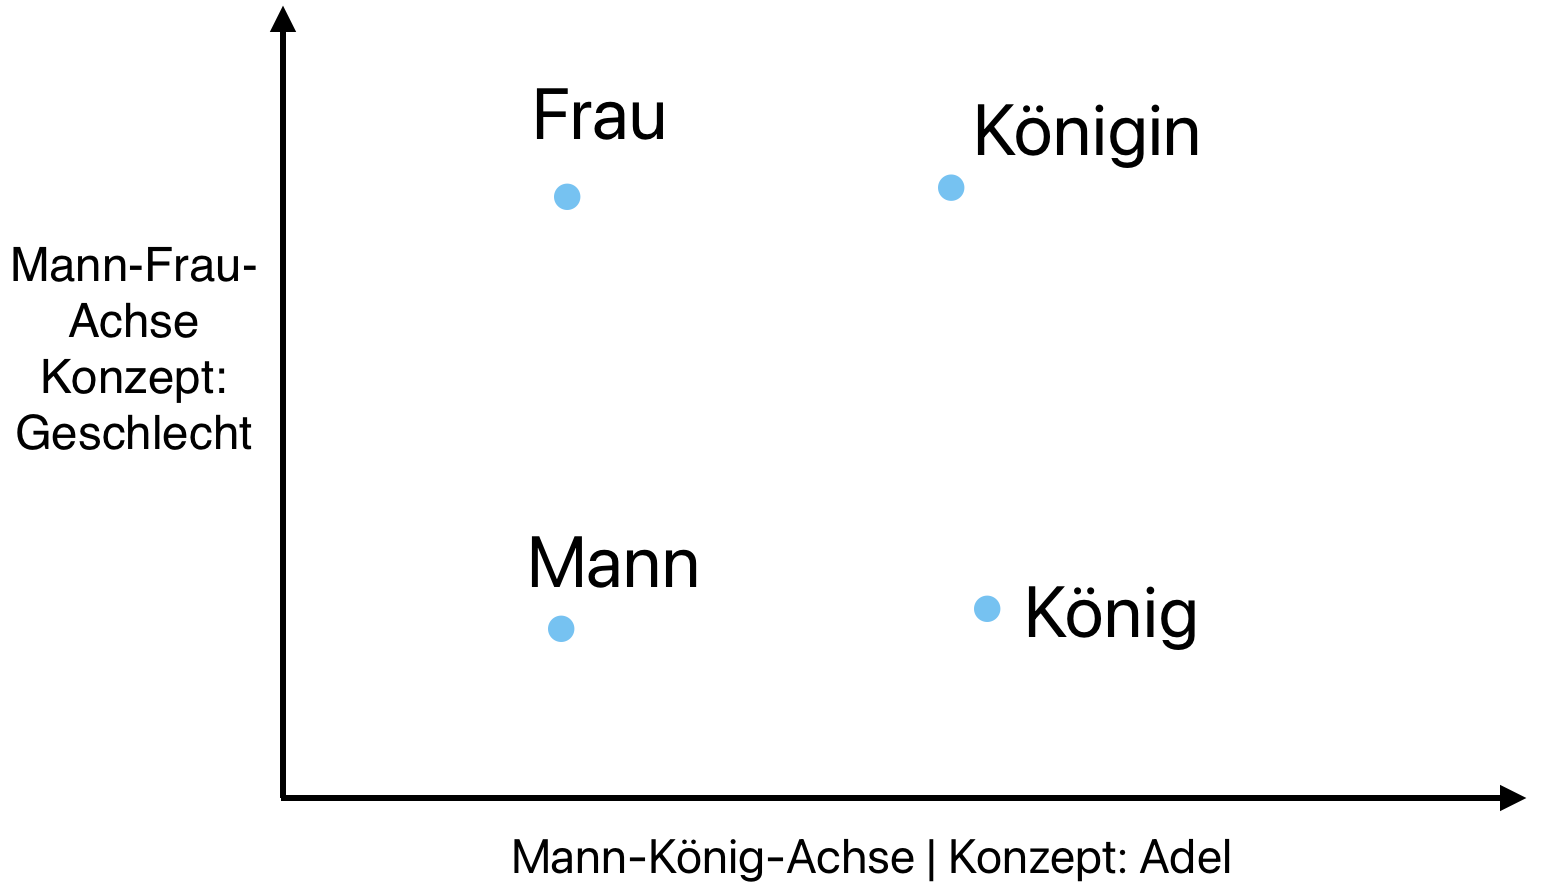
\includegraphics[scale=.23]{"bilder/embeddingspace.png"}
    \caption{Darstellung von einem ausgedachten Emmedding Vektor Raum über zwei Konzept Achsen (Selbst genzeichnet)}
    \label{fig:embeddingspace}
\end{figure}

Um einen Vektor Embedding Raum sinnvoll aufzubauen, ist eine einehitliche Methode zur Embedding Generierung nötig, in der Bedeutungszuweisung von Richtungen kohärent zwischen den Embeddings ist.
Wie bereits erwähnt, wurden \glspl{LLM} für Textverständniss trainiert und können deshalb genutzt werden, um aus einer Text Eingabe ein Ausgabe Vektor Embedding zu erzeugen.
\cite{zhang2023language}

\end{document}